\setcounter{page}{2}

\section{Содержание задания}
Проект представляет собой создание карты города.
В проекте участвуют 16 разработчиков, бюджет проекта~---~50000 рублей, длительность проекта~---~6 месяцев.
Дата начала проекта~---~первый рабочий день марта текущего года.

\section{Сведения о состоянии проекта по базовому плану}

Дата начала проекта в соответствии с базовым планом~---~03.03.2025, дата окончания проекта~---12.08.2025.
Затраты на проект в соответствии с базовым планом составляют 48945 рублей. 

\section{Сведения об актуализации состояния проекта}

По заданию дата отчета~---~11.05.2025.

Произошли следующие изменения:

\begin{itemize}[label=---]
	\item с 10 марта на 2 недели заболел 3D-аниматор, в этот период его заменял художник-дизайнер из расчета 60\% занятости по своим задачам и 40\% занятости по задачам 3D-аниматора с учетом повышения его ставки на 10\% в этот период;
	\item задача <<Разработка 3D графических элементов>> фактически завершилась 19.03;
	\item с 1 апреля изменился график совещаний и состав их участников~---~они стали проводится раз в две недели при участии ведущего программиста, аналитика, мультимедиа корреспондента, веб-дизайнера и технического писателя;
	\item фактическая длительность задач <<Анализ и построение структуры базы объектов>> и <<Программирование средств обработки базы объектов>> оказалась на 20\% больше;
	\item с 1 апреля купили собственный сервер за 4000 рублей и отказались от аренды.
\end{itemize}

Состояние остальных задач соответствует базовому плану проекта.

После актуализации состояния проекта отклонение по длительности проекта составило 0.07 недели~---~проект завершается 13.08, затраты стали меньше на 3053 рубля и составили 45892 рубля.

\section{Задание 1}

Таблица затрат приведена на рисунках~\ref{fig:screen1}~---~\ref{fig:screen3}.

\begin{figure}[H]
	\centering
	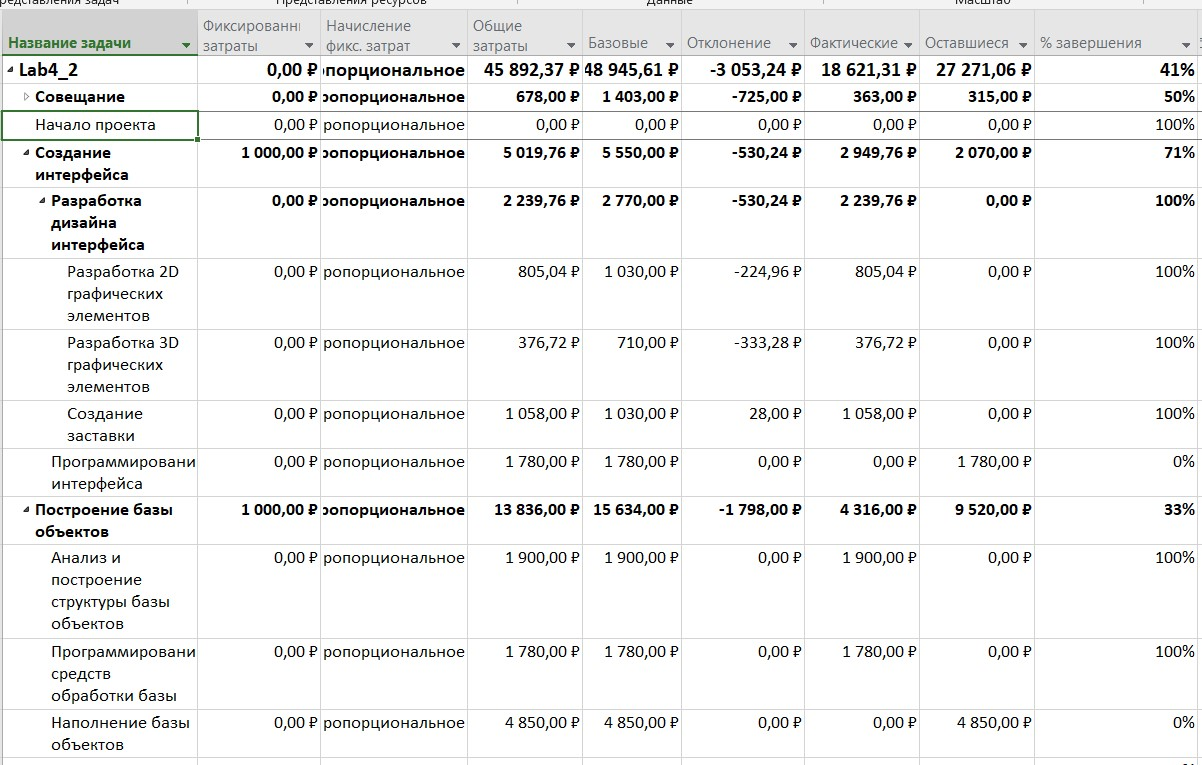
\includegraphics[width=0.9\textwidth]{img/screen1_1.jpg}
	\caption{Таблица затрат}
	\label{fig:screen1}
\end{figure}

\begin{figure}[H]
	\centering
	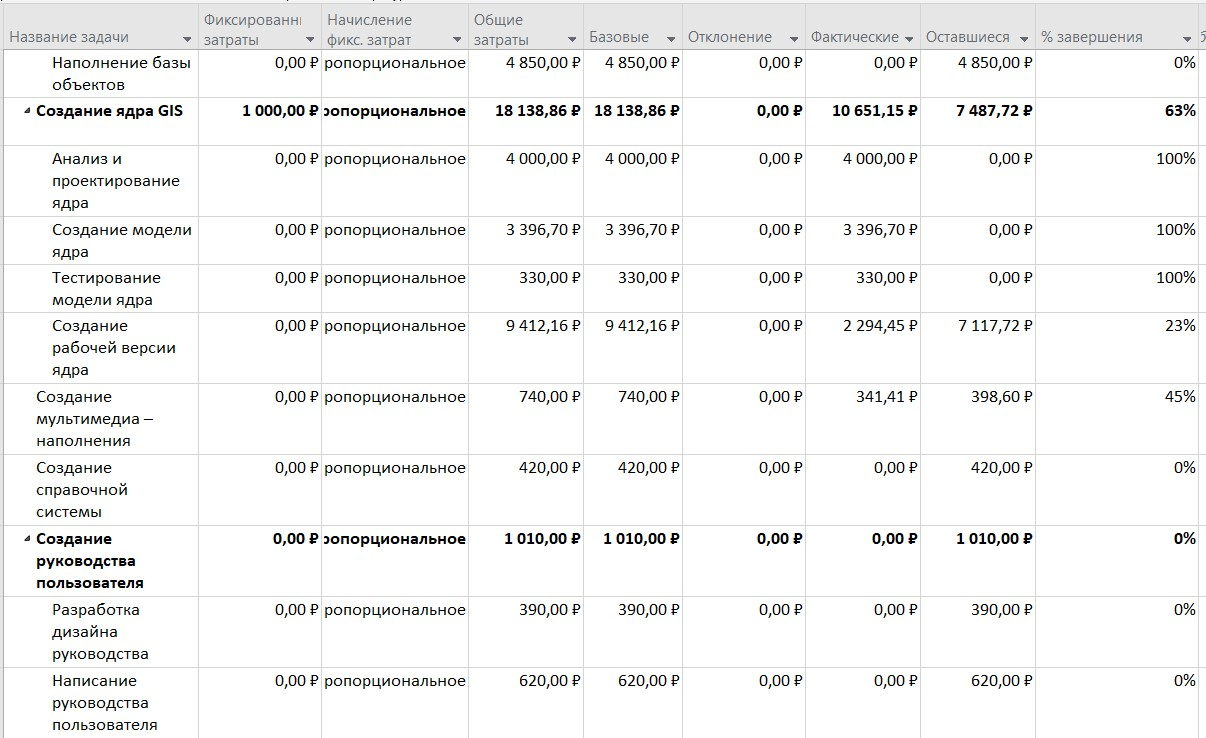
\includegraphics[width=0.9\textwidth]{img/screen1_2.jpg}
	\caption{Таблица затрат}
	\label{fig:screen2}
\end{figure}

\begin{figure}[H]
	\centering
	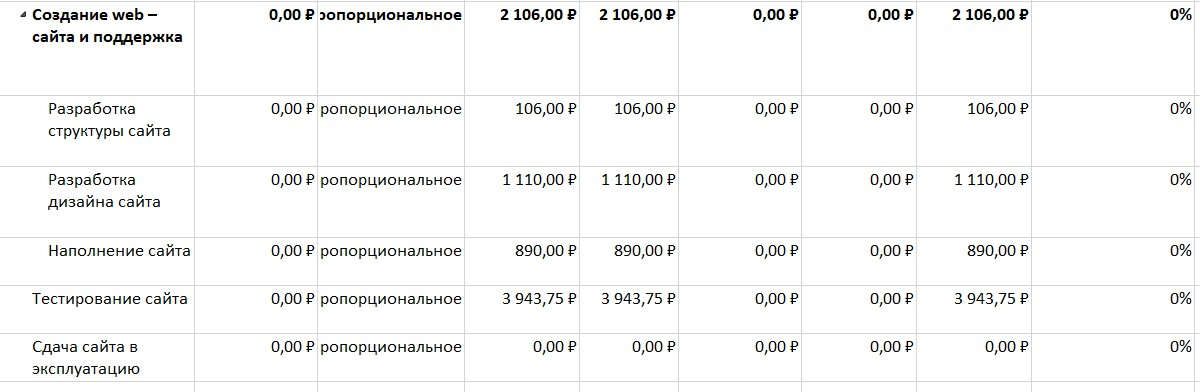
\includegraphics[width=0.9\textwidth]{img/screen1_3.jpg}
	\caption{Таблица затрат}
	\label{fig:screen3}
\end{figure}

Фактические затраты на 11 мая составили 18621 рубль.

Прямые затраты, связанные с выполнением задач:
\begin{itemize}[label=---]
	\item $1000 * 0.71 = 710$ рублей для задачи <<Создание интерфейса>>;
	\item $1000 * 0.33 = 330$ рублей для задачи <<Построение базы объектов>>;
	\item $1000 * 0.63 = 630$ рублей для задачи <<Создание ядра GIS>>.
\end{itemize}

Прямые затраты составляют 1670 рублей ($~9\%$).
Косвенные затраты, связанные с использованием ресурсов составляют $18621 - 1670 = 16951$ рубль ($~91\%$).

Таблица <<Освоенный объем>> приведена на рисунках~\ref{fig:screen4} и~\ref{fig:screen5}.

\begin{figure}[H]
	\centering
	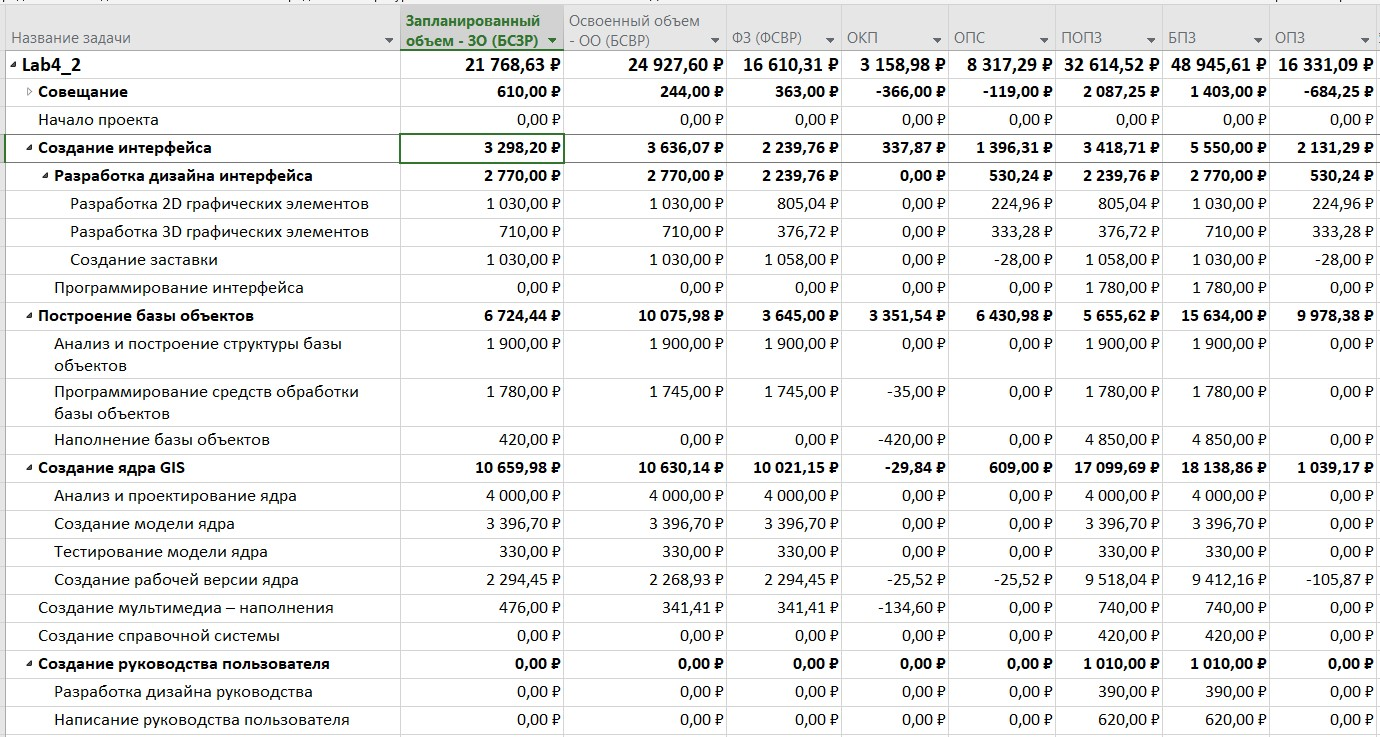
\includegraphics[width=0.9\textwidth]{img/screen2_1.jpg}
	\caption{Освоенный объем}
	\label{fig:screen4}
\end{figure}

\begin{figure}[H]
	\centering
	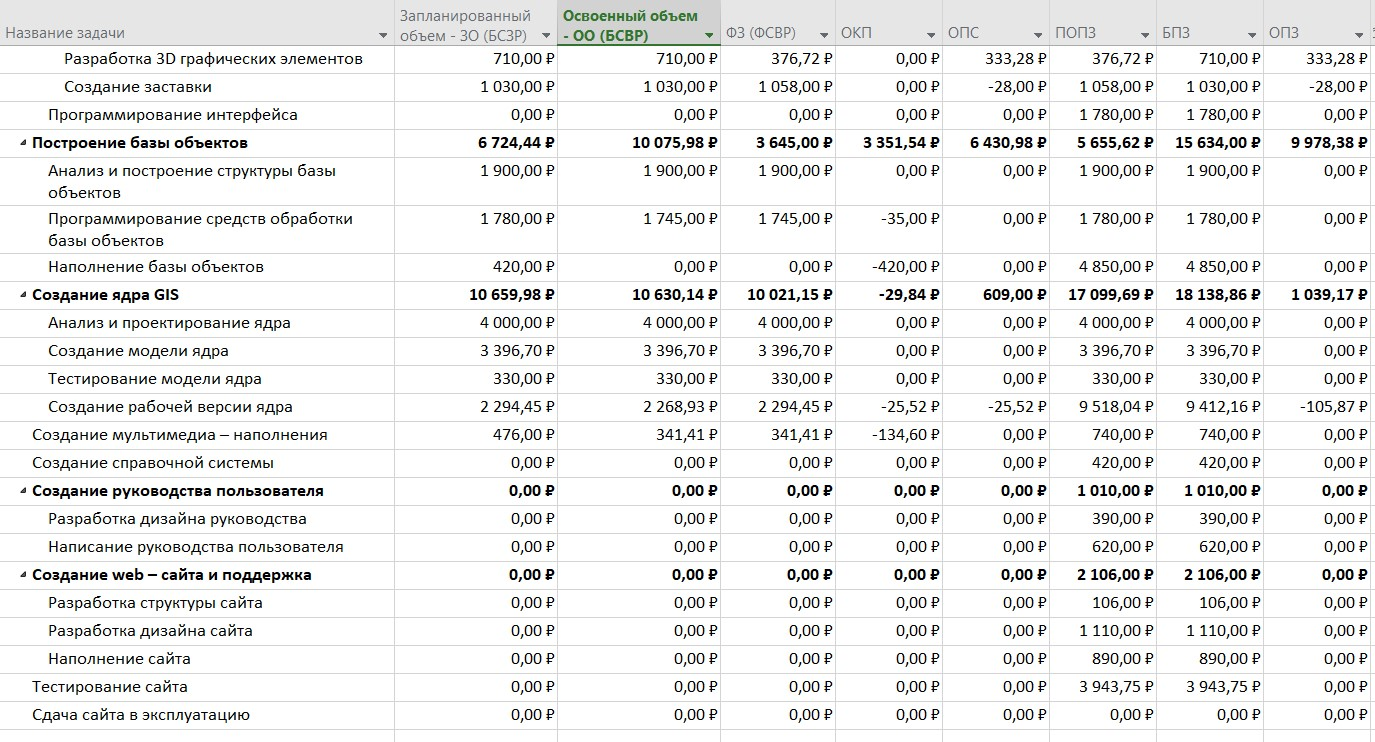
\includegraphics[width=0.9\textwidth]{img/screen2_2.jpg}
	\caption{Освоенный объем}
	\label{fig:screen5}
\end{figure}

Таблица освоенного объема содержит следующие поля:
\begin{itemize}
	\item запланированный объем (ЗО) --- те средства, которые были бы затрачены на выполнение задачи в период с начала проекта до выбранной даты отчета, если бы задача точно соответствовала графику и смете;
	\item освоенный объем (ОО), или базовая стоимость выполненных работ (БСВР) --- те средства, которые были бы затрачены на выполнение задачи с самого начала проекта до выбранной даты отчета, если бы фактически выполненная работа оплачивалась согласно смете, т.е. это фактическое количество рабочих часов, оплачиваемых по сметным ставкам;
	\item фактические затраты (ФЗ) --- средства, фактически потраченные на выполнение задачи в период с начала
	проекта до выбранной даты отчета, т.е. это фактическая стоимость задачи или фактическая ставка, умноженная на фактические часы;
	\item отклонение от календарного плана (ОКП = ОО - ЗО) --- сравнивает сметную стоимость плановой и выполненной работы и позволяет вычислить несоответствие сметы, вызванное исключительно различиями между плановым и фактическим объемом работы;
	\item отклонение по стоимости (ОПС = ОО - ФЗ) --- сравнивает сметную и фактическую стоимость выполненной работы и позволяет выделить несоответствие сметы, вызванные разницей стоимости ресурсов;
	\item предварительная оценка по завершении (ПОПЗ) --- ожидаемые общие затраты для задачи, расчет которых основан на предположении, что оставшаяся часть работы будет выполнена в точном соответствии со сметой;
	\item затраты по базовому плану (БПЗ)--- фиксированные затраты и стоимость ресурсов согласно базовому плану;
	\item отклонение по завершению (ОПЗ = БПЗ - ПОПЗ) --- разность между БПЗ и ПОПЗ.
\end{itemize}

Исходя из таблицы освоенного объема:
\begin{itemize}[]
	\item ЗО $= 21768$ рублей;
	\item ОО $= 24927$ рублей;
	\item ФЗ $= 16610$ рублей;
	\item ОКП $= 3158$ рублей;
	\item ОПС $= 8317$ рублей;
	\item ПОПЗ $= 32614$ рублей;
	\item БПЗ $= 48945$ рублей;
	\item ОПЗ $= 16331$ рубль;
\end{itemize}

ОПС $> 0$, так как затраты на совещания снизились из-за нового состава работников, присутствующих на совещании, а сервер после 1 апреля не требует арендной платы из-за покупки собственного.
ОПЗ $> 0$, то есть перерасход средств отсутствует.

Для совещаний ОКП $= -366$, так как сократилось число совещаний, следовательно трудозатраты на них снизились, а ОПС $= -119$, так как <<Обновленное совещание>> введено как новое событие и не учитывается в освоенном объеме.

Для задачи <<Разработка 2D графических элементов>> ОПС $> 0$, так как художник-дизайнер потратил меньше трудозатрат на эту задачу (89,6 часов вместо 120).

Для задачи <<Разработка 3D графических элементов>> ОПС $> 0$, так как трудозатраты 3D-аниматора на ней снизились с 80 часов до 34 часов из-за его болезни и завершения задачи 19.03.

Для задачи <<Создание заставки>> ОПС $< 0$, так как трудозатраты 3D-аниматора на ней снизились с 120 часов до 113 часов, а художник-дизайнер, не назначенный на эту задачу в базовом плане, потратил на нее 6 часов, работая по повышенной ставке.

Для задачи <<Программирование средств обработки базы объектов>> ОКП $< 0$, так как на момент отчета (11.05) задача не завершена из-за задержки начала задачи на 0.4 недели и задержки окончания задачи на неделю из-за попадания на даты майских праздников.

Для задачи <<Наполнение базы объектов>> ОКП $< 0$, так как на момент отчета (11.05) задача не была начата (по базовому плану она должна была начаться 29.04), что вызвано задержкой предшествующей задачи <<Программирование средств обработки базы объектов>>.

Для вехи <<Построение базы объектов>> основной вклад в то, что ОКП и ОПС $> 0$ вносит покупка собственного сервера и отказ от аренды~---~затраты на аренду сервера снизились до 306 рублей, а процент завершения использования стал 100\%, из-за чего ОО стал равным 6104 рубля, в то время как ЗО равен 2274 рубля.

Для задачи <<Создание рабочей версии ядра>> ОКП $< 0$, так как на момент отчета процент завершения задачи меньше запланированного.

Для задачи <<Создание мультимедиа-наполнения>> ОКП $< 0$, так как на момент отчета процент завершения задачи меньше запланированного в связи с задержкой начала задачи из-за задержки окончания разработки дизайна интерфейса.

По результатам анализа можно сделать вывод, что проект немного отстает от плана, однако не происходит перерасхода средств.

\section{Задание 2}

Согласно отчету о бюджетной стоимости, приведенному на рисунке~\ref{fig:screen6}, самые большие затраты приходятся на 13 неделю года, то есть 24.03 --- 28.03, в течение которой происходит совещание, а также задачи <<Разработка 2D графических элементов>>, <<Создание заставки>>, <<Анализ и построение структуры базы объектов>>, требующая аренду сервера, <<Создание модели ядра>>, то есть одновременно задействованы два самых дорогих члена команды --- ведущий программист и аналитик, а также художник-дизайнер, 3D-аниматор, программисты 1 и 2.

\begin{figure}[H]
	\centering
	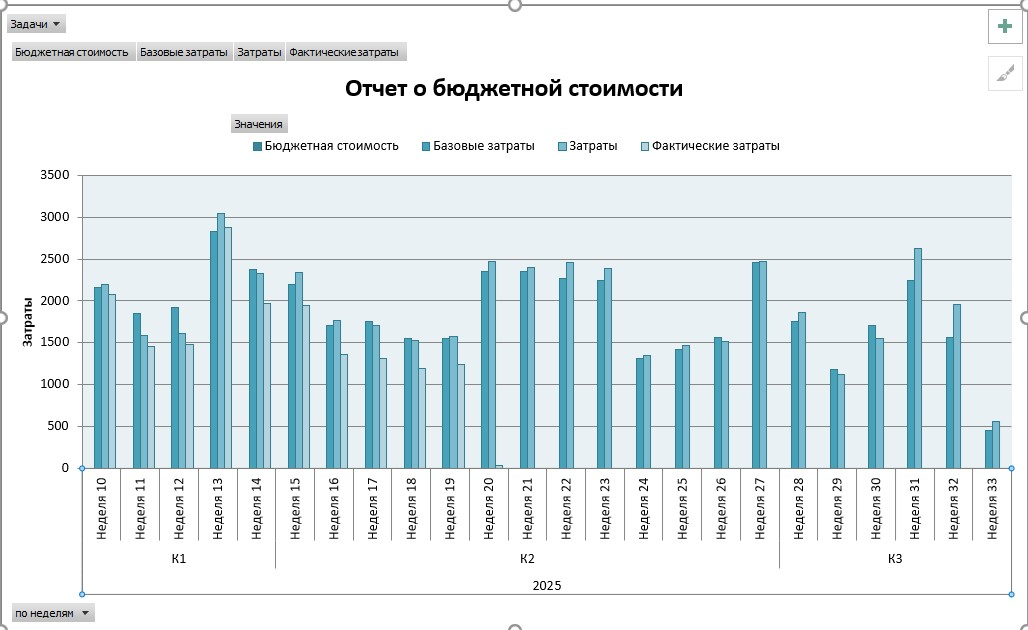
\includegraphics[width=0.9\textwidth]{img/screen3.jpg}
	\caption{Отчет о бюджетной стоимости}
	\label{fig:screen6}
\end{figure}

Отклонения по стоимости задач и ресурсов приведено на рисунках~\ref{fig:screen7} и~\ref{fig:screen8}.

\begin{figure}[H]
	\centering
	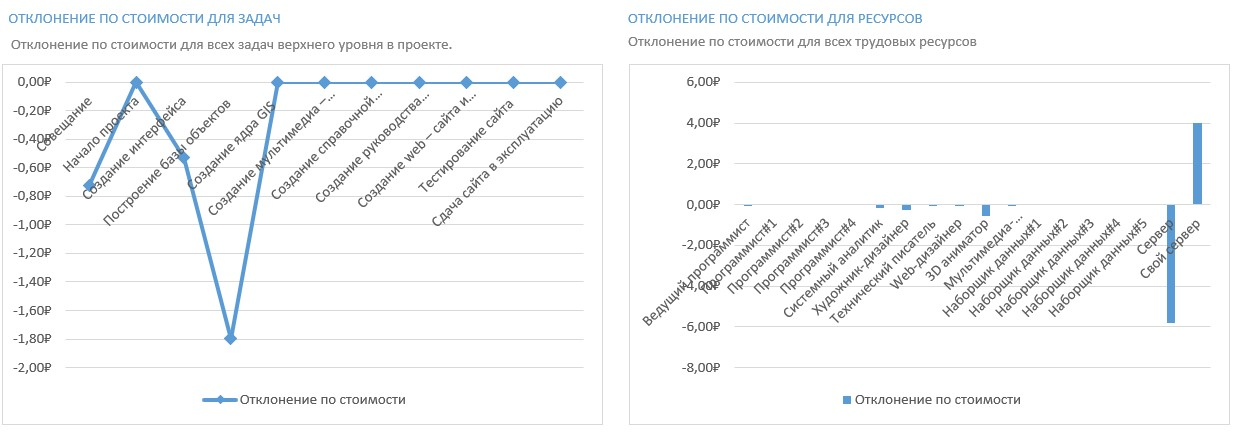
\includegraphics[width=0.9\textwidth]{img/screen4_2.jpg}
	\caption{Графики отклонений стоимости задач и ресурсов}
	\label{fig:screen7}
\end{figure}

\begin{figure}[H]
	\centering
	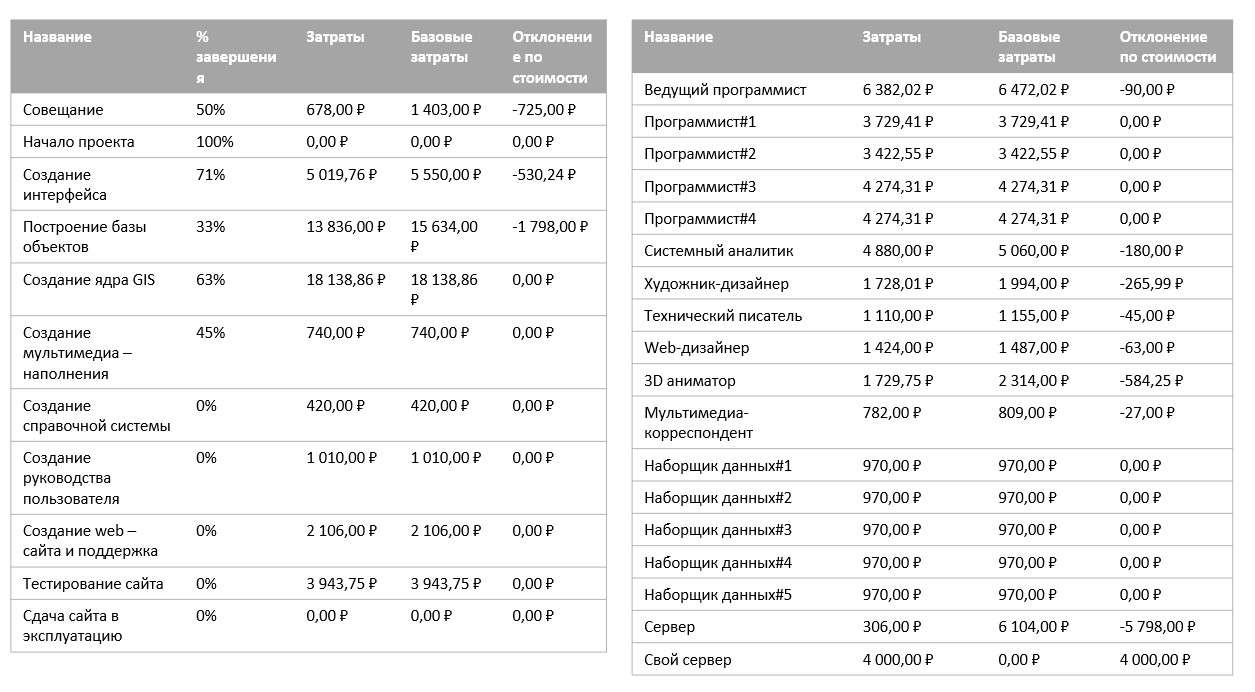
\includegraphics[width=0.9\textwidth]{img/screen4_3.jpg}
	\caption{Таблицы отклонений стоимости задач и ресурсов}
	\label{fig:screen8}
\end{figure}

Основное снижение затрат на ресурсы вызвано изменением графика совещаний и состава их участников.
Это также видно для задачи <<Совещание>> в таблице отклонений стоимости по задачам.
Снижение затрат на задачу <<Построение базы объектов>> вызвано отказом от аренды сервера с 01.04 и покупкой собственного сервера.
Снижение затрат на задачу <<Создание интерфейса>> вызвано завершением задачи <<Разработка 3D графических элементов>> с меньшими трудозатратами, чем планировалось, из-за болезни 3D-аниматора.

\section{Задание 3}

Декомпозиция задач по результатам лабораторной работы №2 представлена на рисунке~\ref{fig:screen9}.

\begin{figure}[H]
	\centering
	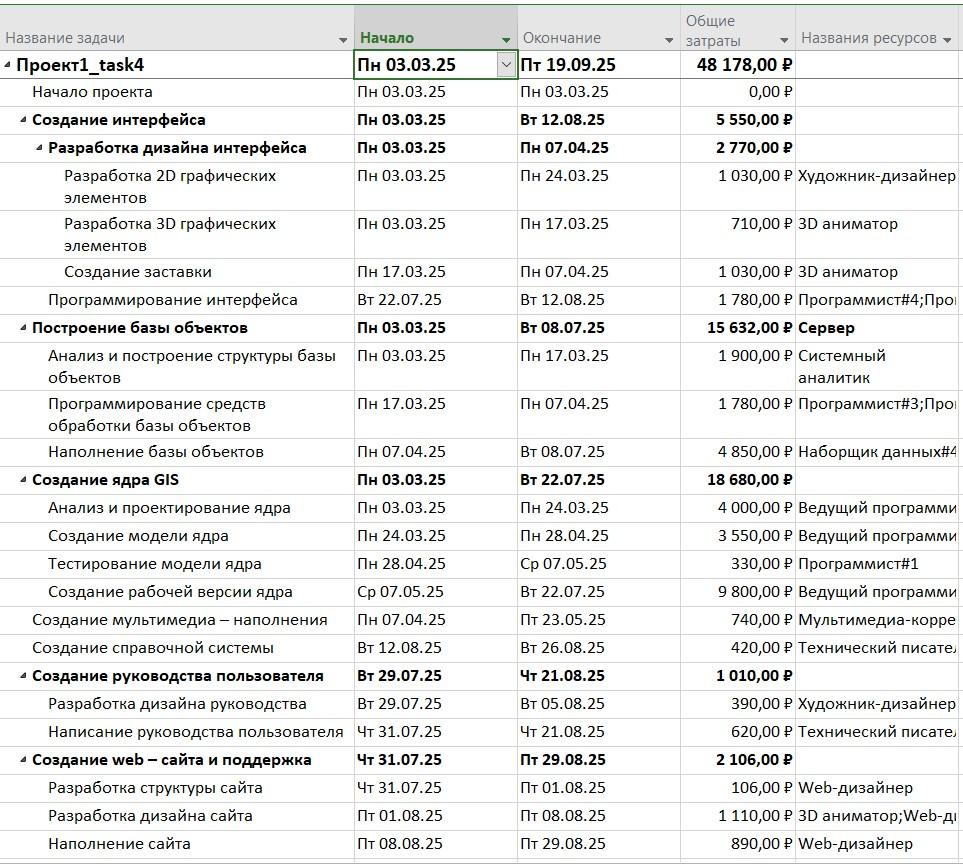
\includegraphics[width=0.9\textwidth]{img/screen5_1.jpg}
	\caption{Декомпозиция задач по результатам лабораторной работы №2}
	\label{fig:screen9}
\end{figure}

Затраты на проект составляют 48178 рублей, проект завершается 19.09.

Новая декомпозиция задач приведена на рисунках~\ref{fig:screen10} и~\ref{fig:screen11}.
Задачи разбиты на этапы проектирования, разработки (включая разработку дизайна, кодирование и наполнение), тестирование и написание документации.

\begin{figure}[H]
	\centering
	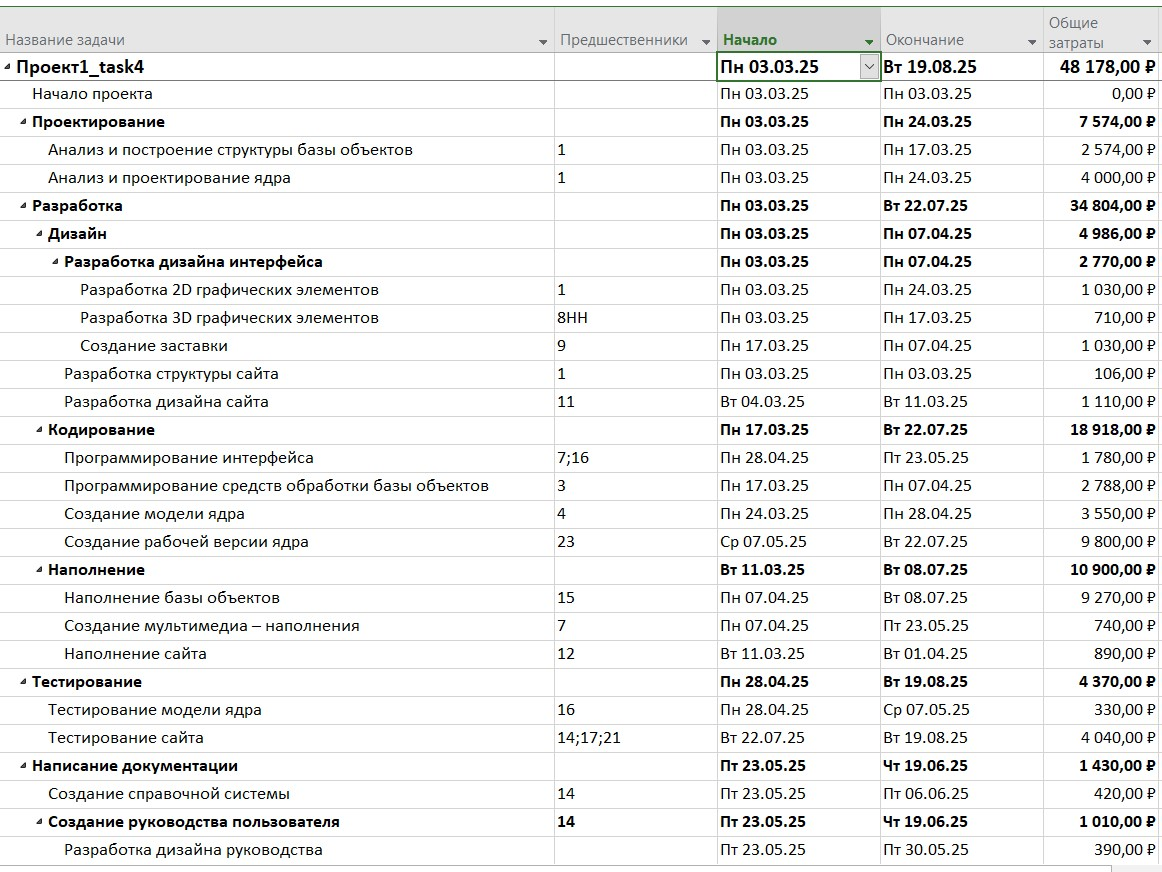
\includegraphics[width=0.9\textwidth]{img/screen5_2.jpg}
	\caption{Новая декомпозиция задач}
	\label{fig:screen10}
\end{figure}

\begin{figure}[H]
	\centering
	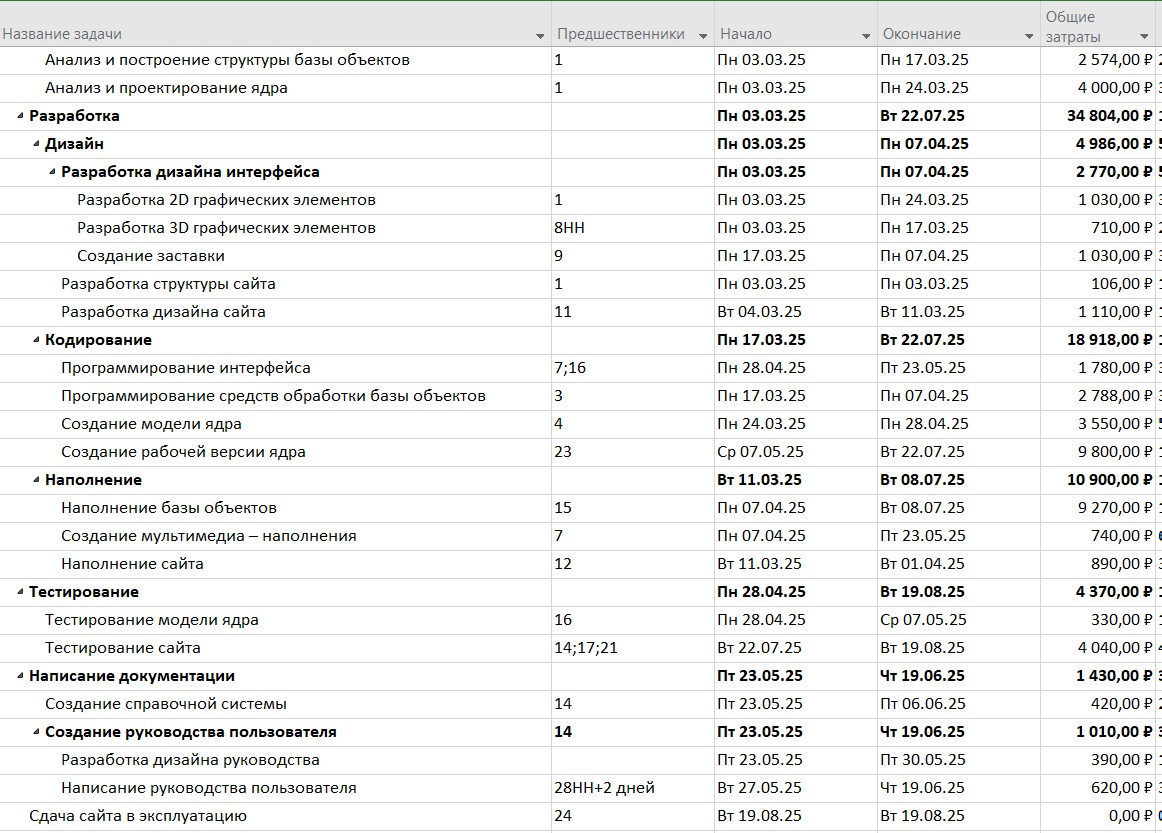
\includegraphics[width=0.9\textwidth]{img/screen5_3.jpg}
	\caption{Новая декомпозиция задач}
	\label{fig:screen11}
\end{figure}

Возникают перегрузки системного аналитика, художника-дизайнера, 3D-аниматора и технического писателя.

Перегрузка системного аналитика вызвана одновременным началом задач <<Анализ и проектирование базы объектов>> и <<Анализ и проектирование ядра>> и наложение на 2 недели.

Перегрузка художника-дизайнера и 3D-аниматора вызвана пересечением задач <<Разработка 2D графических элементов>> для художника и <<Разработка 3D графических элементов>> для аниматора с задачей <<Разработка дизайна сайта>>, начинающихся 03.03 и 04.03.

Перегрузка технического писателя вызвана пересечением задач <<Создание справочной системы>> (длится с 23.05 до 06.06) и <<Написание руководства пользователя>> (с 27.05 до 19.06).

\begin{figure}[H]
	\centering
	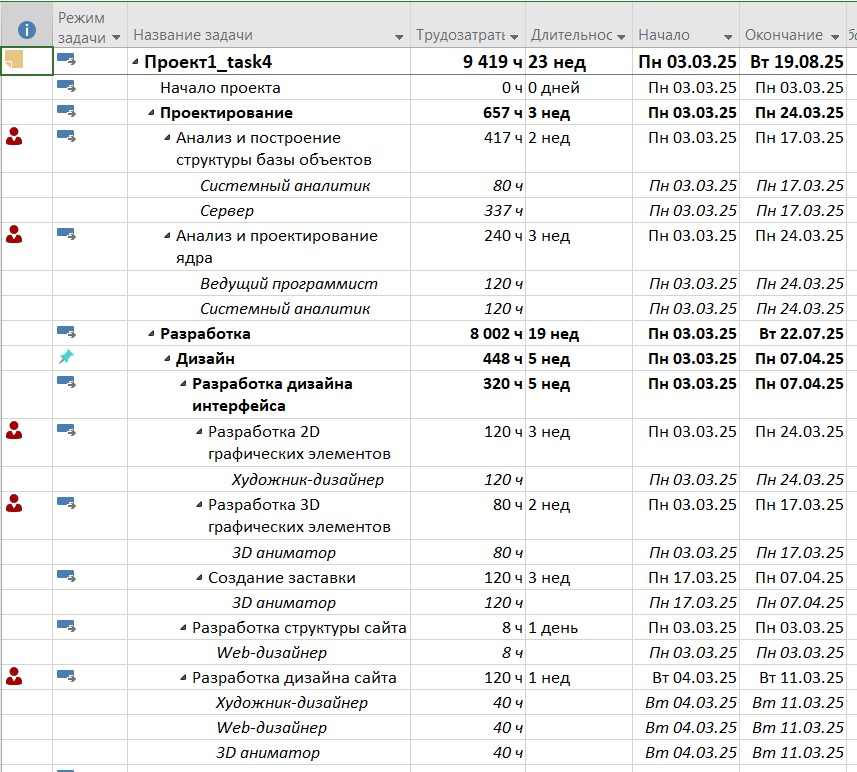
\includegraphics[width=0.9\textwidth]{img/screen5_4.jpg}
	\caption{Перегрузки ресурсов}
	\label{fig:screen12}
\end{figure}

\begin{figure}[H]
	\centering
	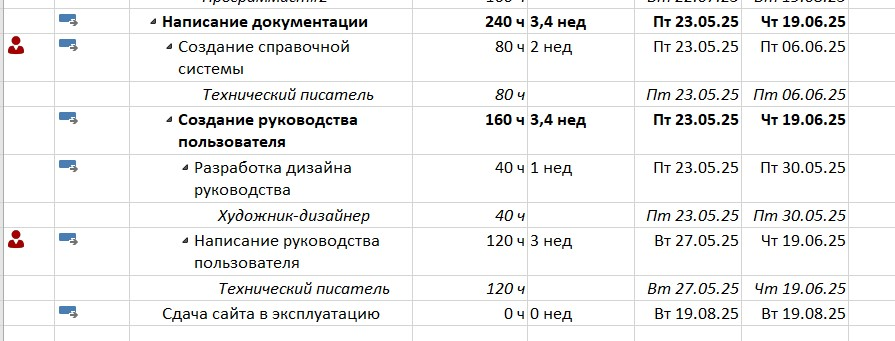
\includegraphics[width=0.9\textwidth]{img/screen5_5.jpg}
	\caption{Перегрузка технического писателя}
	\label{fig:screen13}
\end{figure}

Затраты проекта также составляют 48178 рублей, однако проект завершается на месяц раньше (19.08) из-за одновременного начала задач анализа, выполняющихся параллельно друг другу задач кодирования и параллельности набора данных и написания документации.
